% !TEX root = ./IQF - Minitestes.tex
% IQF - Miniteste 4 resolução

\setcounter{part}{3}
\part{}

% Q2
\setcounter{question}{1}
\begin{questionBox}1m{}
    
    Responda as seguintes questões com base nas constantes do produto de solubilidade e nos dados de potencial de redução padrão fornecidos

    \begin{itemize}
        \begin{multicols}{2}
            \item \(E^{\circ} (\ch{Ag^+/Ag}) = +0.80\,\unit{\volt}\)
            \item \(E^{\circ} (\ch{Cu^+/Cu}) = +0.34\,\unit{\volt}\)
            \item \(K_{ps}(\ch{AgCl}) = 1.6\E-10\)
        \end{multicols}
    \end{itemize}

    Considere a pilha constituida pela acoplamento da seim-célula:

    \begin{center}
        \ch{Cu\sld{}|Cu^+} (\(1.0\E-2\)\,\unit{\molar}) com \ch{AgCl\sat{}|Ag\sld{}}
    \end{center}

    % \begin{center}
    %     \ch{
    %         AgCl\sld{} <> Ag^+\aq{} + Cl^-\sld{}
    %     \\  Ag^+\aq{} + e^- <> Ag\sld{}
    %     \\  Cu\sld{} <> Cu^+\aq{} + e^-
    %     \\  Ag^+\aq{} + Cu\sld{} <> ag\sld{} + Cu^+\aq{}
    %     }
    % \end{center}

    % (i)
    \begin{questionBox}3{}
        
        A 25\,\unit{\celsius} o valor do potencial padrão de reduçã da pilha assim formada será \(E^{\circ}=\,\)\line(1,0){3em}\,\unit{\volt}
        
        \begin{flalign*}
            &
                \Delta E^{\circ}
            =   E^{\circ} (\ch{Ag^+/Ag})
            -   E^{\circ} (\ch{Cu^+/Cu})
            =   (0.80-0.34)\,\unit{\volt}
            =   0.44\,\unit{\volt}
            &
        \end{flalign*}

    \end{questionBox}

    % (ii)
    \begin{questionBox}3{}
        
        Calcule o quociente da reação que ocorre na pilha, \(Q=\,\)\line(1,0){3em}
        
        \begin{flalign*}
            &
                \left.
                \begin{array}{ll}
                &
                    Q
                    =   \ch{[Cu^+]}/\ch{[Ag^+]}
                \,\land\\\land\,&
                    \ch{[Ag^+]}\ch{[Cl^-]}=K_{ps}(\ch{AgCl})
                \,\land\\\land\,&
                    \ch{[Cl^-]}=\ch{[Ag^+]}
                \end{array}
                \right\}
            \implies &\\&
            \implies
                Q
            =   \frac{\ch{[Cu^+]}}{\sqrt{K_{ps}(\ch{AgCl})}}
            =   \frac{1.0\E-2}{\sqrt{1.6\E-10}}
            \cong
                \num{790.569415042094833}
            &
        \end{flalign*}

    \end{questionBox}

    % (iii)
    \begin{questionBox}3{}
        
        A pilha apresenta uma diferença de potencial \(E=\,\)\line(1,0){3em}\,\unit{\volt}

        \sisetup{exponent-mode=scientific}

        \begin{flalign*}
            &
                E 
            =   E^{\circ} - \frac{R\,T}{N\,\mathscr{F}}\,\ln(Q)
            =   0.44 - \frac{\num{8.31446261815324}*(25+273.15)}{1*\num{96485.33212}}\,\ln(\num{790.569415042094833})
            \cong
                \qty{0.268646005666139}{\volt}
            &
        \end{flalign*}
        
    \end{questionBox}
    
    % (iv)
    \begin{questionBox}3{}
        
        A constante de equilíbrio da reação que ocorre na pilha é \(K=\,\)\line(1,0){3em}

        \begin{flalign*}
            &
                % \left.
                %     \begin{array}{ll}
                %     &   k = \exp(N\,\mathscr{F}\,E^{\circ} / R\,T)
                %     \end{array}
                % \right\}
                K
            =   \exp
                \left(
                    N\,\mathscr{F}\,E^{\circ} / R\,T
                \right)
            =   \exp
                \left(
                    1*\num{96485.33212}*0.44 / \num{8.31446261815324}*(25+273.15)
                \right)
            \cong
                \num{27386687.010473627579101}
            &
        \end{flalign*}

    \end{questionBox}

    Considere agora uma nova pilha onde se utilizou uma solução com \(\ch{[Ag^+]}=1\E-10\,\unit{\molar}\) ao invés da solução saturada de \ch{AgCl} no elétodo de prata, mantendo todas as outras condições constantes.

    % (v)
    \begin{questionBox}3{}
        
        A nova pilha assim formada tem uma força eletromotriz de \(E=\,\)\line(1,0){3em}\,\unit{\volt}

        \begin{flalign*}
            &
                \left.
                \begin{array}{ll}
                &
                    E = E^{\circ} - \frac{R\,T}{N\,\mathscr{F}}\,\ln(Q)
                \,\land\\\land\,&
                    Q = \ch{[Ag^+]}/\ch{[Cu^+]}
                \end{array}
                \right\}
            \implies &\\&
            \implies 
                E
            =   E^{\circ} - \frac{R\,T}{N\,\mathscr{F}}
            \,  \ln\left(
                    \frac{\ch{[Ag^+]}}{\ch{[Cu^+]}}
                \right)
            = &\\&
            =   -0.44 - \frac{\num{8.31446261815324}*298}{1*\num{96485.33212}}
            \,  \ln\left(
                    \frac{1.0\E-10}{1.0\E-2}
                \right)
            % \cong &\\&
            \cong
                \qty{3.327479749449477e-2}{\volt}
            &
        \end{flalign*}
        
    \end{questionBox}

    % (vi)
    \begin{questionBox}3{}
        
        No cátodo desta nova pilha ocorre a seguinte semi-reação de redução:
        \begin{enumerate}[label=\alph*)]
            \begin{multicols}{2}
                \item \ch{Cu^+/Cu}
                \item \ch{Ag^+/Ag}
            \end{multicols}
        \end{enumerate}

        \ch{Cu^+/Cu}
        % \ch{Ag^+/Ag}
        
    \end{questionBox}

    % (vii)
    \begin{questionBox}3{}
        
        Enquanto no ânodo a semi-reação de oxidação é:
        \begin{enumerate}[label=\alph*)]
            \begin{multicols}{2}
                \item \ch{Cu/Cu^+}
                \item \ch{Ag/Ag^+}
            \end{multicols}
        \end{enumerate}
        
        % \ch{Cu/Cu^+}
        \ch{Ag/Ag^+}

    \end{questionBox}

\end{questionBox}

% Q3
\begin{questionBox}1{}
    
    A constante cinética de hidrólise do etanoato de metilo a 35\,\unit{\celsius} é 1.82 vezes maior que a 25\,\unit{\celsius}, enquanto que para a hidrólise da sacarose essa relação é de 4.13. Qual a relação entre as energias de ativação destas duas reações?

    \vspace{2ex}

    Selecione uma opção de resposta:

    \vspace{1ex}
    A energia de ativação para a hidrólize do etanoato de metile é \line(1,0){3em} vezes a energia de ativação para a hidrólise da sacarose.
    \begin{enumerate}[label=\alph*)]
        \begin{multicols}{4}
            \item 2.37
            \item 0.42
            \item 0.44
            \item 2.27
        \end{multicols}
    \end{enumerate}

    \begin{flalign*}
        &
            k = A\,\exp\left(\frac{E_a}{R\,T}\right)
        % \implies &\\&
        \implies
            E_a
        =   \frac
                {R\,\unit{\kelvin}\,\ln\frac{k_{35\,\unit{\celsius}}}{k_{25\,\unit{\celsius}}}}
                {(35+273.15)^{-1} - (25+273.15)^{-1}}
        \implies &\\&
        \implies
            \frac{E_{a} (\text{etanoato de metilo})}{E_{a} (\text{sacarose})}
        =   \cfrac
                {
                    \cfrac
                    {R\,\unit{\kelvin}\,\ln\frac{k_{35\,\unit{\celsius}}}{k_{25\,\unit{\celsius}}}}
                    {(35+273.15)^{-1} - (25+273.15)^{-1}}
                }
                {
                    \cfrac
                    {R\,\unit{\kelvin}\,\ln\frac{k_{35\,\unit{\celsius}}}{k_{25\,\unit{\celsius}}}}
                    {(35+273.15)^{-1} - (25+273.15)^{-1}}
                }
        = &\\&
        =   \frac{\ln(1.82)}{\ln(4.13)}
        \cong
            \num[exponent-mode=fixed]{0.422228048014114}
        &
    \end{flalign*}
    
\end{questionBox}

% Q4
\begin{questionBox}1m{}
    
    Os produtos de solubilidade para uma série de iodetos são os seguintes:
    \begin{itemize}
        \begin{multicols}{2}
            \item \(k_{sp} (\ch{TlI}) = 6.5\E-8\)
            \item \(k_{sp} (\ch{AgI}) = 8.3\E-17\)
            \item \(k_{sp} (\ch{PbI2}) = 7.1\E-9\)
            \item \(k_{sp} (\ch{BiI3}) = 8.1\E-19\)
        \end{multicols}
    \end{itemize}

    Quais das seguintes afirmações em relação à ordem de solubilidade estão corretas?
    Selecione uma ou mais opções de resposta:

    \begin{enumerate}[label=\Alph*.]
        \item Em água: \ch{PbI2\,>\,TlI\,>\,AgI\,>\,BiI3}
        \item Numa solução 0.1\,\unit{\molar} do cation: \ch{PbI2\,>\,BiI3\,>\,TlI\,>\,AgI}
        \item Numa solução 0.1\,\unit{\molar} em \ch{NaI}: \ch{PbI2\,>\,BiI3\,>\,AgI\,>\,TlI}
        \item O \ch{AgI} é o sal mais insolúvel da série em duas das condições.
    \end{enumerate}

    \sisetup{
        exponent-mode = scientific,  % scientific/engineering/fixed/false
        % output-exponent-marker = {\,\mathrm{E}},
        round-precision     = 2,
        round-mode          = places,       % figures/places/none
        % exponent-to-prefix  = false,        % 1000 g -> 1 kg
        % round-minimum       = 0.01,
        % fixed-exponent      = -6,
    }

    % (i)
    \begin{questionBox}3{Em àgua}

        \begin{table}[H]\centering
            \begin{tabular}{lccc}
               
                \multicolumn{4}{c}{\ch{XI_n\sld{} <> X + n I}}

            \\\toprule

                \multicolumn{1}{c}{t}
            &   \multicolumn{1}{c}{\ch{XI_n\sld{}}}
            &   \multicolumn{1}{c}{\ch{X}}
            &   \multicolumn{1}{c}{\ch{I}}
               
            \\\midrule
               
                0
            &   -- & 0 & 0
            \\  1
            &   -- & x & n\,x
               
            \\\bottomrule
               
            \end{tabular}
        \end{table}\vspace{-5ex}

        \begin{flalign*}
            &
                \left.
                    \begin{array}{ll}
                    &   \ch{[X]}_1\,\ch{[I]}_1^n = k_{sp} (\ch{XI_n})
                    \,\land\\\land\, &
                        \ch{[X]}_1 = x
                    \,\land\\\land\, &
                        \ch{[I]}_1 = n\,x
                    \end{array}
                \right\}
            \implies
                x = \sqrt[n+1]{k_{sp} (\ch{XI_n})/n^n}
            \implies &\\&
            \implies
                \left\{
                    \begin{array}{llll}
                    &                   x (\ch{[PbI2]}) &= \sqrt[3]{7.1\E- 9/2^2} &\cong \num{0.001210782455002}
                    \,\land\\\land\, &  x (\ch{[TlI ]}) &= \sqrt[2]{6.5\E- 8/1^1} &\cong \num{0.00025495097568}
                    \,\land\\\land\, &  x (\ch{[AgI ]}) &= \sqrt[2]{8.3\E-17/1^1} &\cong \num{0.000000009110434}
                    \,\land\\\land\, &  x (\ch{[BiI3]}) &= \sqrt[4]{8.1\E-19/3^3} &\cong \num{0.00001316074013}
                    \end{array}
                \right.
            &
        \end{flalign*}

    \end{questionBox}

    \begin{questionBox}3{Numa solução 0.1\,\unit{\molar} do cation}

        \begin{table}[H]\centering
            \begin{tabular}{llll}
              
                \multicolumn{4}{c}{\ch{XI_n\sld{} <> X + n\,I}}

            \\\toprule

                \multicolumn{1}{c}{t}
            &   \multicolumn{1}{c}{\ch{XI_n\sld{}}}
            &   \multicolumn{1}{c}{\ch{X}}
            &   \multicolumn{1}{c}{\ch{I}}
               
            \\\midrule
               
                0
            &   -- & 0.1 & 0
            \\  1
            &   -- & 0.1+x & n\,x
               
            \\\bottomrule
               
            \end{tabular}
        \end{table}\vspace{-5ex}

        \begin{flalign*}
            &
                \left.
                    \begin{array}{ll}
                    &                   \ch{[X]}_1\,\ch{[I]}_1^n = k_{sp} (\ch{XI_n})
                    \,\land\\\land\,&   \ch{[X]}_1 = x + 0.1 \cong 0.1 : k_{sp} (\ch{XI_n}) \leq 1\E-3
                    \,\land\\\land\,&   \ch{[I]}_1 = n\,x
                    \end{array}
                \right\}
            \implies &\\&
            \implies 
                x (\ch{XI_n}) \cong \sqrt[n]{k_{sp} (\ch{XI_n})/0.1}/{n} : k_{sp} (\ch{XI_n}) \leq 1\E-3
            \implies &\\&
            \implies
                \left\{
                    \begin{array}{llll}
                    &                   x (\ch{[PbI2]}) &= \sqrt[3]{7.1\E- 9/0.1}/2 &\cong \num{0.002070408874711}
                    \,\land\\\land\, &  x (\ch{[TlI ]}) &= \sqrt[2]{6.5\E- 8/0.1}/1 &\cong \num{0.00080622577483}
                    \,\land\\\land\, &  x (\ch{[AgI ]}) &= \sqrt[2]{8.3\E-17/0.1}/1 &\cong \num{0.000000028809721}
                    \,\land\\\land\, &  x (\ch{[BiI3]}) &= \sqrt[4]{8.1\E-19/0.1}/3 &\cong \num{0.0000177827941}
                    \end{array}
                \right.
            &
        \end{flalign*}

    \end{questionBox}

    \begin{questionBox}3{Numa solução 0.1\,\unit{\molar} em \ch{NaI}}
        
        \begin{table}[H]\centering
            \begin{tabular}{llll}
              
                \multicolumn{4}{c}{\ch{XI_n\sld{} <> X + n\,I}}

            \\\toprule

                \multicolumn{1}{c}{t}
            &   \multicolumn{1}{c}{\ch{XI_n\sld{}}}
            &   \multicolumn{1}{c}{\ch{X}}
            &   \multicolumn{1}{c}{\ch{I}}
               
            \\\midrule
               
                0
            &   -- & 0 & 0.1
            \\  1
            &   -- & x & 0.1
               
            \\\bottomrule
               
            \end{tabular}
        \end{table}\vspace{-5ex}
        
        \begin{flalign*}
            &
                \left.
                    \begin{array}{ll}
                    &                   \ch{[X]}\,\ch{[I]}^n = k_{sp} (\ch{XI_n})
                    \,\land\\\land\,&   \ch{[X]}_1=x
                    \,\land\\\land\,&   \ch{[I]}_1=0.1+x\cong 0.1:k_{sp} (\ch{XI_n})\leq1\E-3
                    \end{array}
                \right\}
            \implies &\\&
            \implies
                x (\ch{XI_n}) \cong k_{sp} (\ch{XI_n}) / 0.1^n
            \implies &\\&
            \implies
                \left\{
                    \begin{array}{llll}
                    &                   x (\ch{[PbI2]}) &= 7.1\E- 9 / 0.1^2 &\cong \num{7.1e-7}
                    \,\land\\\land\, &  x (\ch{[TlI ]}) &= 6.5\E- 8 / 0.1^1 &\cong \num{6.5e-7}
                    \,\land\\\land\, &  x (\ch{[AgI ]}) &= 8.3\E-17 / 0.1^1 &\cong \num{8.3e-16}
                    \,\land\\\land\, &  x (\ch{[BiI3]}) &= 8.1\E-19 / 0.1^3 &\cong \num{8.1e-16}
                    \end{array}
                \right.
            &
        \end{flalign*}

    \end{questionBox}

    \begin{questionBox}3{O \ch{AgI} é o sal mais insolúvel da série em duas das condições.}
        
        Em agua e em 0.1\,\unit{\molar} do cátion.
        
    \end{questionBox}
    
\end{questionBox}

% Q5
\begin{questionBox}1{}
    
    Qual a concentração de amónia aquosa (\ch{NH3}) em \unit{\mole\per\cubic{\deci\meter}\,(\molar)} necessária para iniciar a precipitação de \ch{Mg(OH)2} de uma solução 0.041\,\unit{\molar} em \ch{Mg2^+}?
    (Na resposta indique apenas o resultado numérico)

    \begin{itemize}
        \begin{multicols}{2}
            \item \(k_{b } (\ch{NH3})     = 1.8\E- 5\)
            \item \(k_{sp} (\ch{Mg(OH)2}) = 1.2\E-11\)
        \end{multicols}
    \end{itemize}
    
    % \begin{center}
    %     \ch{ NH3\aq{} + H2O\lqd{} <> NH4^+\aq{} + OH^-\aq{} \\ Mg(OH)2\sld{} <> Mg^+\aq{} + 2 OH^-\aq{}}
    % \end{center}

    \begin{table}[H]\centering
        \begin{tabular}{c*{4}{l}}
            
                \multicolumn{5}{c}{\ch{NH3\aq{} + H2O\lqd{} <> NH4^+\aq{} + OH^-\aq{}}}

            \\\toprule
            
                \multicolumn{1}{c}{t}
            &   \multicolumn{1}{c}{\ch{NH3\aq{}}}
            &   \multicolumn{1}{c}{\ch{H2O\lqd{}}}
            &   \multicolumn{1}{c}{\ch{NH4^+\lqd{}}}
            &   \multicolumn{1}{c}{\ch{OH^-\lqd{}}}
            
            \\\midrule
            
                0 & \ch{[NH3]_0} & -- & 0 & 0
            \\  1 & \ch{[NH3]_1} & -- & \ch{[OH^-]_1} & \ch{[OH^-]_1}
            
            \\\bottomrule

        \end{tabular}

        \begin{tabular}{c*{3}{l}}

                \multicolumn{4}{c}{\ch{Mg(OH)2\sld{} <> Mg^+\aq{} + 2 OH^-\aq{}}}

            \\\toprule

                \multicolumn{1}{c}{t}
            &   \multicolumn{1}{c}{\ch{OH^-\aq{}}}
            &   \multicolumn{1}{c}{\ch{Mg^+\lqd{}}}
            &   \multicolumn{1}{c}{\ch{NH4^+\lqd{}}}

            \\\midrule

                1 & \ch{[OH^-]_1} & \ch{[Mg^+]_1} & --

            \\\bottomrule
            
        \end{tabular}
    \end{table}\vspace{-5ex}

    \begin{flalign*}
        &
            \left.
                \begin{array}{ll}
                &                   \ch{[NH3]}_0 = \ch{[NH3]}_1 + \ch{[OH^-]}_1
                \,\land\\\land\,&   \ch{[NH3]}_1 = \ch{[OH^-]}_1^2/k_b (\ch{[NH3]})
                \,\land\\\land\,&   \ch{[OH^-]}_1 > \sqrt{k_{sp} (\ch{Mg(OH)2})/\ch{[Mg^+]}_1}
                \end{array}
            \right\}
        \implies &\\&
        \implies
            \ch{[NH3]}_0 
        =   \frac{\left(\sqrt{k_{sp} (\ch{Mg(OH)2})/\ch{[Mg^+]}_1}\right)^2}{k_b (\ch{[NH3]})} + \sqrt{k_{sp} (\ch{Mg(OH)2})/\ch{[Mg^+]}_1}
        = &\\&
        =   \frac{1.2\E-11/0.041}{1.8\E-5} + \sqrt{1.2\E-11/0.041}
        \cong
            \num{3.336814105699205e-5}
        &
    \end{flalign*}

\end{questionBox}

% Q6
\begin{questionBox}1{}
    
    Qual a constante de equilíbrio, a 25\,\unit{\celsius}, para a seguinte reação:

    \begin{center}
        \ch{2 Ag^+ + Sn <> Sn^{2+} + 2 Ag}
    \end{center}
    \begin{itemize}
        \begin{multicols}{2}
            \item \(E^{\circ} (\ch{Ag^{ +}/Ag}) = +0.800\,\unit{\volt}\)
            \item \(E^{\circ} (\ch{Sn^{2+}/Sn}) = -0.136\,\unit{\volt}\)
        \end{multicols}
    \end{itemize}

    Utilize notação científica na resposta (exemplo: 0.00010 será \(1.0\E-4\))

    \begin{flalign*}
        &
            \left.
                \begin{array}{ll}
                &                   k = \exp\left(\frac{-\Delta G^{\circ}}{R\,T}\right)
                \,\land\\\land\,&   \Delta G^{\circ} = -n\,\mathscr{F}\,E^{\circ}
                \end{array}
            \right\}
        % \implies &\\&
        \implies 
            k 
        =   \exp\left(\frac{n\,\mathscr{F}\,E^{\circ}}{R\,T}\right)
        = &\\&
        =   \exp\left(\frac{2*\num{96485.33212}\,(0.800-(-0.136))}{\num{8.31446261815324}*(25+273.15)}\right)
        \cong
            \num{4.398958514350037e31}
        &
    \end{flalign*}

\end{questionBox}

\begin{questionBox}1{}
    
    A reação do violeta de cristal (VC) com o ion hidroxilo é uma reação elementar bimolecular, com uma velocidade que obedece a uma cinética de 2\textsuperscript{a} ordem global, correspondendo à expressão: \(v=-\odv{[VC]}{t} = k\,\ch{[OH^-][VC]}\). A reação foi realizada em condições tais que a reação apresenta uma aparente cinética de 1\textsuperscript{a} ordem. A concentração do VC ao longo do tempo foi seguida por espectroscopia de UV-Vis a 22\,\unit{\celsius} e 40\,\unit{\celsius} e os resultados experimentais estão representados no gráfico abaixo:

    \begin{figure}[H]\centering
        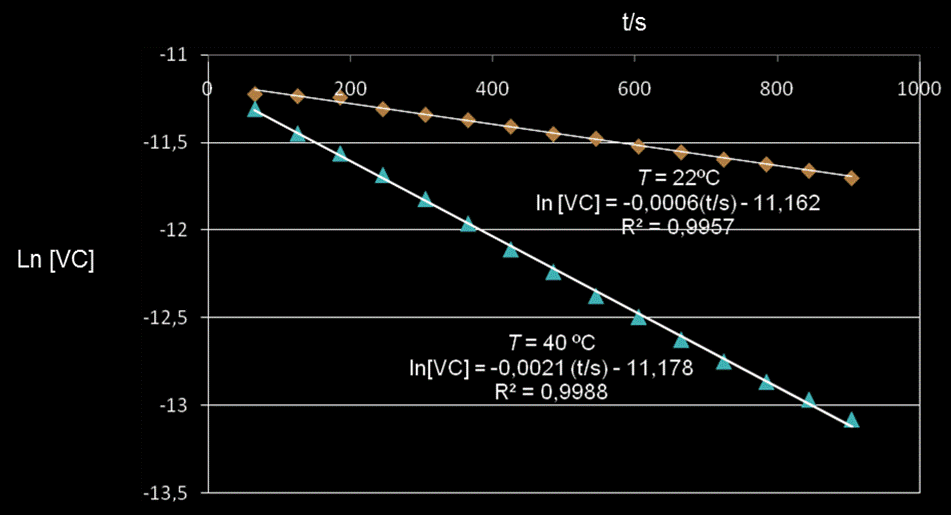
\includegraphics[width=\textwidth]{resources/IQF - Miniteste 4 Q7 img1.png}
    \end{figure}

    Sabendo que a concentração do ion hidroxilo em ambas as misturas rescionais foi 0.01\,\unit{\molar}, calcule a velocidade da reação a 40\,\unit{\celsius} ao fim de 2.5\,\unit{\minute}.
    (responda em \unit{\molar\per\second}, não escreva a unidade na resposta indique só o valor, tolerância 5\%)

    

    \begin{flalign*}
        &
            \left.
                \begin{array}{ll}
                &   v = k\,\ch{[OH^-][VC]}
                \,\land\\\land\,&
                    k\,\ch{[OH^-]} = -(-0.0021)
                \,\land\\\land\,&
                    \ch{[VC]}_{t,40\,\unit{\celsius}} = \exp(-0.0021\,t-11.178)
                \end{array}
            \right\}
        \implies &\\&
        \implies 
            v 
        =   k\,\ch{[OH^-]}\,\exp(-0.0021\,t-11.178)
        = &\\&
        =   0.0021\,\exp(-0.0021\,(2.5*60)-11.178)
        \cong
            \num{2.142263134458894e-8}
        &
    \end{flalign*}

\end{questionBox}

% Q8
\begin{questionBox}1m{}
    
    Recorrendo a uma tabela de potenciais de eletrodos padrões, indique se cada uma das semi-células se comporta como ânodo ou cátodo quando acoplata com um eletrodo padrão de hidrogênio para formar uma célula galvânica e calcule a diferença de potencial da célula.

    \subsubsection*{Dados}
    \begin{itemize}
        \begin{multicols}{2}
            \item \(k_{sp} (\ch{AgBr}) = 5.2\E-13\)
            \item \(E^\circ (\ch{Pb^{+2}/Pb})     = -0.13\,\unit{\volt}\)
            \item \(E^\circ (\ch{Ag^{+ }/Ag})     =  0.8 \,\unit{\volt}\)
            \item \(E^\circ (\ch{Sn^{+4}/Sn^{+2}})=  0.13\,\unit{\volt}\)
        \end{multicols}
    \end{itemize}

    \subsubsection*{Opções}
    \begin{itemize}
        \begin{multicols}{2}
            \item Cátodo, 0.139\,\unit{\volt}
            \item Ânodo,  0.038\,\unit{\volt}
            \item Cátodo, 0.311\,\unit{\volt}
            \item Ânodo,  0.235\,\unit{\volt}
        \end{multicols}
    \end{itemize}

    % \begin{table}[H]\centering
    %     \begin{tabular}{lr}
            
    %         \\\toprule
            
    %             \multicolumn{1}{c}{Especies}
    %         &   \multicolumn{1}{c}{\(E^\circ/\unit{\volt}\)}
            
    %         \\\midrule
            
    %             \ch{Pt^{2+}/Pt} & 1.20
            
    %         \\\bottomrule
            
    %     \end{tabular}
    %     \caption{Tabela de potenciais de eletrodos padrões}
    % \end{table}

    \sisetup{
        exponent-mode = fixed,
        % scientific-notation = engineering,  % scientific/engineering/fixed/false
        % output-exponent-marker = {\,\mathrm{E}},
        round-precision     = 3,
        % round-mode          = places,       % figures/places/none
        % exponent-to-prefix  = false,        % 1000 g -> 1 kg
        % round-minimum       = 0.01,
        % fixed-exponent      = 0,
    }

    \begin{questionBox}3{\ch{Pt|Sn^{4+}} (0.2\,\unit{\molar}), \ch{Sn^{2+}} (0.1\,\unit{\molar})}
        \begin{flalign*}
            &
                E = E^\circ - \frac{R\,T}{N\,\mathscr{F}}\ln(Q)
            = &\\&
            =   0.13\,\unit{\volt} - \frac{\num{8.31446261815324}*(25+273.15)}{2*\num{96485.33212}}\,\ln\left(\frac{0.1}{0.2}\right)\,\unit{\volt}
            \cong
                \num{0.138904369389852}
            &
        \end{flalign*}
    \end{questionBox}

    \begin{questionBox}3{\ch{Pt|Sn^{4+}} (\(1.0\E-6\)\,\unit{\molar}), \ch{Sn^{2+}} (0.5\,\unit{\molar})}
        \begin{flalign*}
            &
                E = E^\circ - \frac{R\,T}{N\,\mathscr{F}}\ln(Q)
            = &\\&
            =   -0.13\,\unit{\volt} - \frac{\num{8.31446261815324}*(25+273.15)}{2*\num{96485.33212}}\,\ln\left(\frac{1.0\E-6}{0.5}\right)\,\unit{\volt}
            \cong
                \num{3.857367967058308e-2}
            &
        \end{flalign*}
    \end{questionBox}

    \begin{questionBox}3{\ch{Pb|Pb^{2+}} (\(2.00\E-4\)\,\unit{\molar})}
        \begin{flalign*}
            &
                E = E^\circ - \frac{R\,T}{N\,\mathscr{F}}\ln(Q)
            = &\\&
            =   0.13\,\unit{\volt} - \frac{\num{8.31446261815324}*(25+273.15)}{2*\num{96485.33212}}\,\ln(2.00\E-4)\,\unit{\volt}
            \cong
                \num{239.414329983771234e-3}
            &
        \end{flalign*}
    \end{questionBox}

    \begin{questionBox}3{\ch{Ag|AgBr\sat{}}, \ch{KBr} (\(1\E-4\)\,\unit{\molar})}
        \begin{flalign*}
            &
                \left.    
                    \begin{array}{ll}    
                    &   E = E^\circ - \frac{R\,T}{N\,\mathscr{F}}\ln(Q)
                    \,\land\\\land\,&
                        Q = \ch{[Ag^+]}^2
                    \,\land\\\land\,&
                        \ch{[Ag^+]} = k_{sp} (\ch{AgBr}) / \ch{[Br^+]}
                    \end{array}
                \right\}
            \implies &\\&
            \implies 
                E 
            =   E^\circ - \frac{R\,T}{N\,\mathscr{F}}\ln\left(\left(\frac{k_{sp} (\ch{AgBr}) }{ \ch{[Br^+]} }\right)^2\right)
            = &\\&
            =   -0.8 - \frac{\num{8.31446261815324}*(25+273.15)}{2*\num{96485.33212}}\,\ln\left(\left(\frac{5.2\E-13}{ 1\E-4 }\right)^2\right)
            \cong
                \num{0.490075854998289}
            &
        \end{flalign*}
    \end{questionBox}
    
\end{questionBox}

% % Q9
% \begin{questionBox}1{}
    
%     A lei da velocidade para a reação:
%     \begin{center}
%         \ch{2 NO\gas{} + Cl2\gas{} -> 2 NOCl\gas{}}
%     \end{center}

%     é \(v=k\,\ch{[NO][Cl2]}\)

%     Foi proposto para esta reação um mecanismo envolvendo os seguintes passos reacionais:

%     \begin{center}
%         \ch{
%             NO\gas + Cl2\gas{} -> NOCl2\gas{}
%         \\  NOCl2\gas{} + NO\gas{} -> 2NOCl\gas{}
%         }
%     \end{center}

%     Assumindo que o mecanismo está correto escolha a afirmação verdadeira (selecione uma opção de resposta):
%     \begin{enumerate}[label=\Alph*.]
%         \begin{multicols}{n}
%             \item A reação é de 1\textsuperscript{a} ordem e o 1\textsuperscript{o} passo do mecanismo é o determinante da velocidade da reação.
%             \item 
%             % A. A reacção é de 1ª ordem e o 1ºpasso do mecanismo é o determinante da velocidade da reacção.
%             % B. A velocidade da reacção não depende da concentração do intermediário NOCl2 e o primeiro passo do mecanismo é mais lento que o segundo.
%             % C. A reacção é de segunda ordem e o segundo passo do mecanismo é o determinante da velocidade da reacção.
%             % D. O primeiro passo do mecanismo, onde está envolvido o catalizador NOCl2 é mais rápido que o segundo.
%         \end{multicols}
%     \end{enumerate}
    
% \end{questionBox}

% Q11
\setcounter{question}{10}
\begin{questionBox}1m{}
    
    A reação do violeta de cristal (VC) com o ion hidroxilo é uma reação elementar bimolecular, com uma velocidade que obedece a uma cinética de 2\textsuperscript{a} ordem global, correspondendo à expressão: \(v=-\adif{\ch{VC}}/\adif t = k\,\ch{[OH^-][VC]}\). Quando \ch{[OH^-]}\,>>\,\ch{[VC]}, podemos escrever a seguinte expressão \(v=-\odif{\ch{[VC]}}/\odif{t} = k'\ch{[VC]},\,k'=k\ch{[OH^-]}\)
    
    \vspace{1ex}
    
    A concentração do VC ao longo do tempo foi seguida por espectroscopia de UV-Vis a 22\,\unit{\celsius} e 40\,\unit{\celsius} e os resultados experimentais estão representados no gráfico abaixo:

    \begin{figure}[H]\centering
        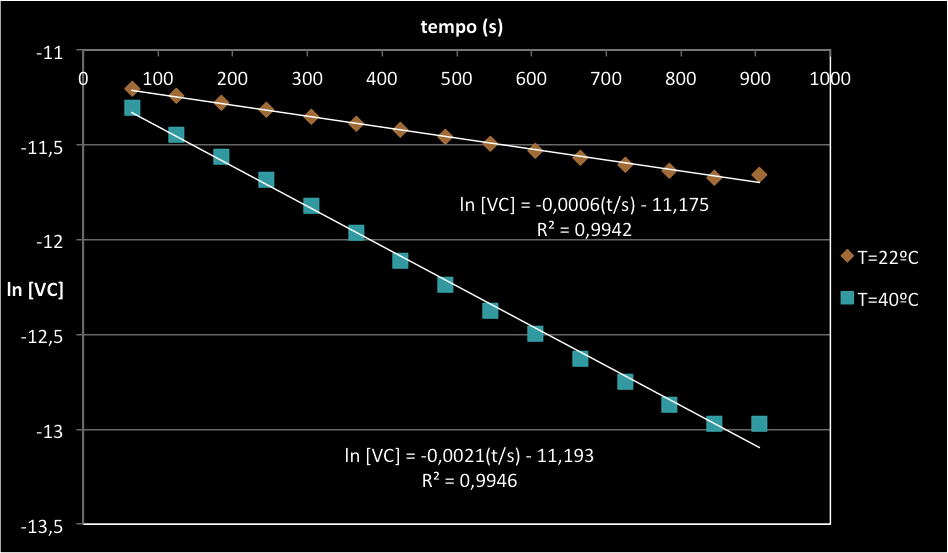
\includegraphics[width=\textwidth]{resources/IQF - Miniteste 4 Q11 img1.png}
    \end{figure}

    \setcounter{subquestion}{1}
    \begin{questionBox}2{}
        
        Calcule o tempo necessário para reduzir a concentração de violeta de cristal a 20\% do seu valor inicial, a 22\,\unit{\celsius}, \(t=\line(1,0){3ex}\)\,\unit{\second}

        \begin{flalign*}
            &
                \left.
                    \begin{array}{ll}
                    &   t = -(\ln\ch{[VC]} + 11.175)/6\E-4
                    \,\land\\\land\,&
                        \ch{[VC]}_t = 20\%\,\ch{[VC]}_0
                    \end{array}
                \right\}
            \implies &\\&
            \implies 
                t 
            =   -(\ln\left(20\%\,\exp(-11.175)\right) + 11.175)/6\E-4
            \cong   
                \num{2682.396520723500624}
            &
        \end{flalign*}

    \end{questionBox}

    \begin{questionBox}2{}
        
        Sabendo que a concentração do ion hidroxilo em ambas as misturas reacionais foi 0.01\,\unit{\molar}, calcule a velocidade da reação a 22\,\unit{\celsius} ao fim de 8\,\unit{\minute}, \(v=\line(1,0){3ex}\)\,\unit{\molar\per\second}
        
        \begin{flalign*}
            &
                \left.
                    \begin{array}{ll}
                    &   v = k\,\ch{[OH^-][VC]}
                    \,\land\\\land\,&
                        k\,\ch{[OH^-]} = -(-6\E-4)
                    \,\land\\\land\,&
                        \ch{[VC]}_(t) = \exp(-6\E-4\,t - 11.175)
                    \end{array}
                \right\}
            \implies &\\&
            \implies
                v_{8\,\unit{\min}}
            =   6\E-4\,\exp(-6\E-4\,(8*60) - 11.175)
            \cong
                \num{6.307156456641828e-9}
            &
        \end{flalign*}

    \end{questionBox}

    \begin{questionBox}2{}
        
        A energia de ativação da reação é \line(1,0){3ex}\,\unit{\joule\per\mole}
        
        \begin{flalign*}
            &
                \left.
                    \begin{array}{ll}
                    &   E_a = -R\,(22+273.15)\,\ln(k_{22\,\unit{\celsius}}/A)
                    % &   k = A\,\exp\frac{E_a}{R\,T}
                    \,\land\\\land\,&
                        k_{22\,\unit{\celsius}} = k'_{22\,\unit{\celsius}}/\ch{[OH^-]}
                    \,\land\\\land\,&
                        \ch{[OH^-]} = k'_{40\,\unit{\celsius}}/k_{40\,\unit{\celsius}}
                    \,\land\\\land\,&
                        k_{40\,\unit{\celsius}} = A\,\exp\left(\frac{-E_a}{R\,(40+273.15)}\right)
                    \end{array}
                \right\}
            \implies &\\&
            \implies
                E_a
            =   \frac
                    {R\,\ln(k'_{40\,\unit{\celsius}}/k'_{22\,\unit{\celsius}})}
                    {295.15^{-1}-313.15^{-1}}
            =   \frac
                    {\num{8.31446261815324}\,\ln(2.1\E-3/0.6\E-3)}
                    {295.15^{-1}-313.15^{-1}}
            \cong
                \num{53484.235298377733728}
            &
        \end{flalign*}

    \end{questionBox}

    \begin{questionBox}2{}
        
        A constante cinética da reação de hidroxilação do violeta de cristal a 28\,\unit{\celsius} é, \(k=\line(1,0){3ex}\)\,\unit{\per\molar\per\second}
        
        \begin{flalign*}
            &
                \left.
                    \begin{array}{ll}
                    &   k_{28\,\unit{\celsius}} = A\,\exp\left(-E_a/R(28+273.15)\right)
                    \,\land\\\land\,&
                        A = k_{22\,\unit{\celsius}}/\exp\left(-E_a/R(22+273.15)\right)
                    \,\land\\\land\,&
                        k_{22\,\unit{\celsius}} = k'_{22\,\unit{\celsius}}/\ch{[OH^-]}
                    \,\land\\\land\,&
                        E_a 
                    =   \frac
                            {R\,\ln(k'_{40\,\unit{\celsius}}/k'_{22\,\unit{\celsius}})}
                            {295.15^{-1}-313.15^{-1}}
                    \end{array}
                \right\}
            \implies &\\&
            \implies 
                k_{28\,\unit{\celsius}} 
            % = &\\&
            =   \frac{k'_{22\,\unit{\celsius}}}{\ch{[OH^-]}}
            \,* &\\&
            *\,
                \exp
                \left(
                    \frac
                        {\ln(k'_{40\,\unit{\celsius}}/k'_{22\,\unit{\celsius}})}
                        {295.15^{-1}-313.15^{-1}}
                    \left(
                        (22+273.15)^{-1}
                    -   (28+273.15)^{-1}
                    \right)
                \right)
            = &\\&
            =   \frac{0.6\E-3}{0.01}
            \,  \exp
                \left(
                    \frac
                        {\ln(2.1\E-3/0.6\E-3)}
                        {295.15^{-1}-313.15^{-1}}
                    \left(
                        (295.15)^{-1}
                    -   (301.15)^{-1}
                    \right)
                \right)
            \cong &\\&
            \cong
                \num{9.262619074109325e-2}
            &
        \end{flalign*}

    \end{questionBox}
    
\end{questionBox}